\documentclass[bibliography=totocnumbered]{scrartcl}
\usepackage{imakeidx}
\usepackage{ragged2e}
\usepackage{setspace} % Um den Zeilenabstand zu ändern.
\usepackage{gensymb}
%\usepackage{authblk}
% \usepackage{minitoc} % for the chpaters
\usepackage{wasysym}
%\usepackage{SI}
\usepackage{array} % Verwendung von Matrizen
\usepackage{booktabs} % Schöne Tabellen beziehungsweise sie sehen damit professioneller aus.
\usepackage{tabulary} % Ähnlich wie tabularx, ermöglicht aber das ändern der Ausrichtung der Spalten.
\usepackage{tabularx} % Tabellen mit automatischen Zeilenumbruch.
\usepackage{enumitem}
\usepackage{physics}
\usepackage[T1]{fontenc}% fontec und inputenc ermöglichen
\usepackage{graphicx}%Für Grafiken
\usepackage{rotating} % lässt Grafiken rotieren
\usepackage{mathtools}% mathematische Werkzeuge
\usepackage{amsmath}% Mathetools
\usepackage{amsfonts}% Mathetools
\usepackage{amssymb}% Symbole wie Natürliche Zahlen
\usepackage{geometry}
%\usepackage{bibtex} 
\usepackage{tablefootnote}% Fußnoten in Tabellen
\usepackage{float}% für eingebundene Bilder
\usepackage{fancyhdr} % Seiten schöner gestalten, insbesondere Kopf- und Fußzeile
\usepackage{ulem} 
\usepackage{dcolumn}% Align table columns on decimal point
\usepackage{bm}% bold math
\usepackage[ngerman]{babel} % Worttrennung nach der neuen Rechtschreibung und deutsche Bezeichnungen. babelfunktion wird wegen Literatur gebraucht.
\usepackage{subfloat} % Was macht diese Packet?
\usepackage{caption} % Unter-/Überschriften für Bilder, Grafiken und Tabellen
\usepackage{subcaption}
\usepackage{txfonts}
\usepackage{titling}% Titel
\usepackage[style=alphabetic]{biblatex} %biblatex mit alphabetic laden. alphbetic=Zitationsstil
\usepackage{bookmark}
\usepackage[printonlyused]{acronym}
\usepackage{amsthm}
\usepackage{pdfpages}
\usepackage{tikz}
\usepackage[siunitx,americanvoltages, europeanresistors,americancurrents]{circuitikz}
\usepackage{listings}
\usepackage{abstract}
\usepackage[per-mode = fraction]{siunitx}
\usepackage{hyperref}
\newcommand{\R}{\mathbb{R}} % reelle Zahlen
\newcommand{\N}{\mathbb{N}} % natürliche Zahlen
\newcommand{\C}{\mathbb{C}} % komplexe Zahlen
\newcommand{\Q}{\mathbb{Q}} % rationale Zahlen
\newcommand{\Z}{\mathbb{Z}} % ganze Zahlen
\newcommand{\F}{\mathbf{F}} % Kraft
\newcommand{\E}{\mathbf{E}} % Energie
\newcommand{\V}{\mathbf{v}} % Geschwindigkeit
\newcommand{\B}{\mathbf{B}} % magnetischer Fluss
\newcommand{\J}{\mathbf{j}} % Stromdichte ?
\newcommand{\D}{\mathbf{D}} % elektrische Induktion
\newcommand{\HH}{\mathbf{H}} % magnetische Feldstärke
\newcommand{\M}{\mathbf{M}} % Magnetisierung
\newcommand{\p}{\mathbf{P}}
\newcommand{\rr}{\mathbf{r}}
\newcommand{\vp}{\varphi}
\newcommand{\ve}{\varepsilon}
\newcommand{\vcc}[1]{\left(\begin{matrix}#1\end{matrix}  \right)}
\newcommand{\m}[1]{\left\lbrace #1\right\rbrace}
\newcommand{\los}{\noindent\textbf{Lösung}:}
\newcommand{\rang}[2]{\text{Rang}(#1)=#2}
\newcommand{\vpe}{\frac{1}{4\pi\ve_0}}
\newcommand{\qvpe}{\frac{q}{4\pi\ve_0}}
\newcommand{\geg}{\ac{geg.}}
\newcommand{\ges}{\ac{ges.}}

\newcommand{\kommando}[1]{$\backslash$\textit{#1}}
\newcommand{\com}[1]{$\backslash$\textit{#1}$\left\lbrace\ldots\right\rbrace$}
\newcommand{\Com}[2]{$\backslash$\textit{#1}$\left\lbrace #2\right\rbrace$}
\newcommand{\NeuKommando}[2]{$\backslash \textit{#1} \left\lbrace \backslash \textit{#2}\right\rbrace$}
\newcommand{\latex}{\LaTeX $\;$}


% si unitx
\DeclareSIUnit\litre{l}

\hypersetup{
	colorlinks=true,
	linkcolor=blue,
	filecolor=magenta,      
	urlcolor=cyan,
	citecolor=lime!50!black,
	filecolor=red
}
%\addbibresource{} %Bibliographiedateien laden
\addbibresource{bib.bib}

\geometry{a4paper, left=25mm, right=25mm, top=30mm, bottom=30mm}
\lhead{\thedate}
\rhead{GPR}
\lhead{\thetitle}
\pagestyle{fancy}

\usetikzlibrary{patterns}
\usetikzlibrary{3d}
\makeindex[title=Stichwortverzeichnis,intoc
,options= -s Index-Formatierung.ist
]
\author{Ben J. F.}
\allowdisplaybreaks

\lstset
{ %Formatting for code in appendix
    basicstyle=\footnotesize,
    numbers=left,
    stepnumber=1,
    showstringspaces=false,
    tabsize=2,
    breaklines=true,
    breakatwhitespace=false,
}

\date{12.05.2021}

\title{M12 Saitenschwingung}

\rfoot{M12}

\begin{document}
	\newgeometry{left=14mm, right=13.5mm, top=60mm, bottom=30mm}
	\begin{titlepage}
		\begin{center}
			{\huge{Grundpraktikum}}\\\vspace*{15mm}
			{\huge{\textbf{\thetitle}}}\\\vspace*{20mm}
			{\theauthor}\\\vspace*{10mm}
			{\thedate}\\\vspace*{40mm}
			\vspace{1.5cm}
			
			
			
		\end{center}
	\end{titlepage}
	\makeatother
	\restoregeometry
	\newpage
	
	\tableofcontents
	\listoffigures 
	\listoftables
	\newpage
	
	
	
	\section{Versuchsbeschreibung}
	% Versuchziel: Was will ich mit dem Versuch erreichen?
	% Aufgabenstellung
	% theoretische Einführung: Wie sieht die Physik dahinter aus (Knapp fassen)? Welche Formeln verwende ich? Wie ist der Versuch aufgebaut (Skizze, Abbildungen etc)? Welche Einheiten kommen vor?
	\begin{figure}[H]
	    \centering
	    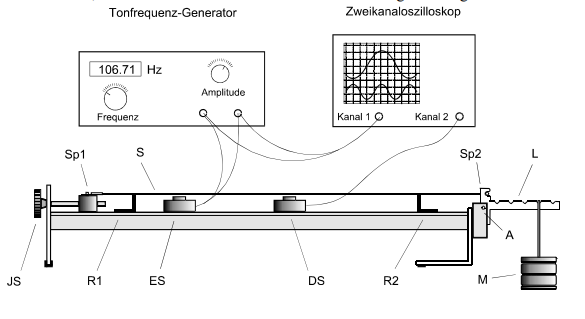
\includegraphics[width=\linewidth]{fotos/gpr1/M12-Versuchsaufbau.png}
	    \caption{Versuchaufbau; Sp1,Sp2=Einspannstellen; R1,R2=Reiter; M=Massestück; L=Lasthebel; JS=Justierschraube; ER=Erregerspule; DR=Detektorspule}							% Bildunterschrift
		\label{Abb: Versuchaufb}							% für Textverweise
	\end{figure}
	
	Das Ziel des Versuchs ist es, die transversalle Schwingung einer Saite zu untersuchen. Dabei betrachten wir die Schwingung als stehende Welle mit Ober- und Grundschwingungen. Im Veruch untersuchen wir den linearen Zusammenhang von der Resonanzfrequenz $ f_{n} $ mit der Anzahl $ n $ an Schwingungsbäuchen, unterschiedlichen Längen $ l $ und unterschiedlichen Zugspannung $ \sqrt{F_{0} }$. Für die Resonanzfrequenz verwenden wir die Gleichung:
	\begin{equation}\label{eq: Resonanzfrequenz}
		f_{n}^{trans}=\dfrac{n}{2l}\sqrt{\dfrac{F_{0}}{\mu}}
	\end{equation}
	Die Phasengeschwindigkeit, welche wir benötigen, ist folgendermaßen definiert:
	\begin{equation}\label{eq: Phasengeschwindigkeit}
		c^{trans}=\sqrt{\dfrac{F_{0}}{\mu}}
	\end{equation}
	Für ein tieferes theoretisches Verständnis ist das Material \textit{M12-Saitenschwingung} hinzu zu ziehen.\\
	\\
  	Eine Stahlsaite ist zwischen zwei Einspannstellen eingespannt. Durch zwei Reiter können wir die Länge der Saite, die schwingt, einstellen. Die Saite wird durch eine Erregerspule angeregt. Knoten und Bäuche der schwingenden Saite können mit der Detektorspule ausfindig gemacht werden, welche dann auf dem Zweikanaloszilloskop angezeigt werden.\footnote{Wenn der zweite Kanal nichts anzeigt, handelt es sich um einen Knoten. Wenn wir einen Schwingungsbauch gefunden haben, sind sich die Applituden von Kanal 1 und 2 ähnlich.} Die Saite wird durch die Zugspannung $ F_{0} $ gespannt, welche durch den Lastenarm und an diesem befestigten Massen hervorgerufen wird. Den genauen Aufbau können wir in Abb. (\ref{Abb: Versuchaufb}) betrachten.
	
	\newpage
	\section{Versuchdurchführung \\und Versuchauswertung}
	% übersichtliche Darstellung der Messdaten, Rechenergebnisse (chronologische Reihenfolge), Grafiken etc.
	
	\subsection{Resonanzfrequenz in Abhängigkeit der Schwingungsbäuche}
	\begin{table}[H]
    \centering
		\caption{Messreihe: Resonanzfrequenz in Abhängigkeit der Schwingungsbäuche}
	\begin{tabular}{|c|c|}
		\hline
		$ f_{n} $ [Hz] & $ n $ \\
		\hline
		78.5$\pm$0.8& 1 \\
		\hline
		157.00$\pm$1.6& 2 \\
		\hline
		234.80$\pm$2.4& 3 \\
		\hline
		314.30$\pm$3.0& 4 \\
		\hline
		393.40$\pm$4.0& 5 \\
		\hline
		472.80$\pm$5.0& 6 \\
		\hline
		552.30$\pm$6.0& 7 \\
		\hline
		631.20$\pm$6.0& 8 \\
		\hline
		710.90$\pm$7.0& 9 \\
		\hline
	\end{tabular}
	\label{tab: n}	
\end{table}
	Unsere Messergebnisse aus dem ersten Teilversuch stehen in der Tabelle (\ref{tab: n}). Die Unsicherheiten von $ f_{n} $ haben wir nach der Frequenzgenauigkeit aus Abb. (\ref{Abb: Agaben}) berechnet:
	\begin{equation}\label{eq: Unsicherheit von f_n}
		u_{f_{n}}=0.01\cdot f_{n}+0.02
	\end{equation}
	Für die lineare Regression haben wir die folgende Gleichung verwendet:
	\begin{equation}\label{eq: Regression 1}
		f_{n}=a\cdot n+b
	\end{equation}
	Wobei $ a $ der Anstieg ist und durch den Vergleich mit der Glg. (\ref{eq: Resonanzfrequenz}) können wir den Anstieg $ a $ wie folgt definieren:
	\begin{equation}\label{eq: Anstieg 1}
		a=\dfrac{\sqrt{\dfrac{F_{0}}{\mu}}}{2l}
	\end{equation}
	Unser Ergebnis für den Anstieg $ a $ und den Achsenabschnitt $ b $ sind wie folgt: 
	\begin{align}\label{eq: Regressionparameter 1}
		a=78.84\pm 0.11 \hspace{3mm}\text{Hz}\\
		b=-0.51\pm 0.26  % möglicher Fehler: f_n nicht quadriert und b sollte FH/(mu*2*l) sein
	\end{align}
	Unsere Messwerte und der Fit mit den eben benannten Regressionsparametern sind in der Abb. (\ref{Abb: Regression 1}) enthalten.\\
	Die Phasengeschwindigkeit $ c^{trans} $ berechen wir aus Glg. (\ref{eq: Anstieg 1}) und Glg. (\ref{eq: Phasengeschwindigkeit}):
	\begin{align}
		a=\dfrac{c}{2l}\\
		\Leftrightarrow c=2al
	\end{align}
	Sodass wir für $ c^{trans} $ herausbekommen:
	\begin{equation}\label{eq: c_trans ergebnis}
		c=(94.61\pm0.20) \hspace{3mm} \text{ms$ ^{-1} $}
	\end{equation}
	\newpage
	
	\subsection{Resonanzfrequenz in Abhängigkeit der Länge}
	\begin{table}[H]
    \centering
		\caption{Messreihe Resonanzfrequenz $ f_{1} $ in Abhängigkeit von Länge $ l $}
		\begin{tabular}{|c|c|}
			\hline
			$ f_{1} $ [Hz] & $ l $ [m] \\
			\hline
			235.7$ \pm $2.4& 0.2$ \pm $0.007 \\
			\hline
			187.0$ \pm $1.9& 0.25$ \pm $0.007 \\
			\hline
			156.5$ \pm $1.6& 0.3$ \pm $0.007 \\
			\hline
			134.5$ \pm $1.4& 0.35$ \pm $0.007 \\
			\hline
			117.2$ \pm $1.2& 0.4$ \pm $0.007 \\
			\hline
			103.93$ \pm $1.1& 0.45$ \pm $0.007 \\
			\hline
			94.0$ \pm $1.0& 0.5$ \pm $0.007 \\
			\hline
			78.8$ \pm $0.8& 0.55$ \pm $0.007 \\
			\hline
			72.6$ \pm $0.7& 0.6$ \pm $0.007 \\
			\hline
		\end{tabular}
	\label{tab: l}
\end{table}
	Unsere Messergebnisse aus dem zweiten Teilversuch stehen in der nebigen Tabelle (\ref{tab: l}). Die Unsicherheit von $ l $ haben wir folgendermaßen berechnet: 
	\begin{align}\label{eq: l unsicherheit}
		u_{l}=\sqrt{u_{Anfangswert}^{2}+u_{Endwert}^{2}}
	\end{align}
Auf diese Fehlerfortpflanzung kommen wir, weil wir $ l $ folgendermaßen berechnet haben:
\begin{equation}\label{eq: Länge}
	l=l_{Endwert}-l_{Anfangswert},\text{ mit } l_{Anfangswert}<l_{Endwert}
\end{equation}
Dabei haben wir eine Ableseungenauigkeit von $ 0.5 $ mm angenommen.\\
Wie wir auf die Unsicherheiten von $ f_{1} $ kommen, haben wir bereits in Glg. (\ref{eq: Unsicherheit von f_n}) erwähnt.\\
Die lineare Regression der Daten befindet sich in Abb. (\ref{Abb: Regression 2}). Für die Fitgerade haben wir uns für die folgende Form entschieden:
\begin{equation}\label{eq: Regression 2}
	f_{1}=\dfrac{c}{2l}+b
\end{equation}
	Dabei bezeichnet $ c $ die Phasengeschwindigkeit, $ b $ den Achsenabschnitt und $ l $ bezeichnet die Länge, welche wir in der Tabelle  (\ref{tab: l}) haben. Für $ c $ und b haben wir folgende Werte herausbekommen:\footnote{Wir haben uns für genau dieses vorgehen entschieden, weil wir von Python direkt die Phasengeschwindigkeit mit Unsicherheit bekommen und uns damit etwas Rechenarbeit ersparrt haben.}
	\begin{align}
		c=(96.9\pm 1.5)\text{ ms$ ^{-1} $}\\
		b=(-5.5\pm 2.2) \text{ Hz}
	\end{align}
Der Anstieg ist \begin{equation}
	a=\dfrac{c}{2}=(48.45\pm 0.75)\text{ ms$ ^{-1} $}
\end{equation}
Vergleichen wir die Phasengeschwindigkeiten von diesem Teilversuch und dem ersten Teilversuch:
\begin{align}\label{eq: Vergleich}
		c=(94.61\pm0.20) \hspace{3mm} \text{ms$ ^{-1} $}\\
		c=(96.9\pm 1.5)\text{ ms$ ^{-1} $}
\end{align}
so sehen wir, dass die zweite Phasengeschwindigkeit etwas höher ist mit einer größeren Unsicherheit. Das lässt darauf schließen, dass wir bei dem zweiten Teilversuch etwas ungenauer gearbeitet haben.
\newpage

	\subsection{Resonanzfrequenz in Abhängigkeit der Zugspannung}
	\begin{table}[H]
    \centering
		\caption{Messreihe zwischen $ f_{1} $ und Masse $ m $}
		\begin{tabular}{|c|c|}
			\hline
			$ f_{1} $ [Hz]& $ m $ [kg] \\
			\hline
			77.88 $ \pm $0.8& 1.00$ \pm $ 0.000011\\
			\hline
			76.39 $ \pm $0.8& 0.95$ \pm $0.00001 \\
			\hline
			71.76 $ \pm $0.7&  0.80$ \pm $0.00001\\
			\hline
			69.11 $ \pm $0.7& 0.75$ \pm $ 0.000009\\
			\hline
			63.95 $ \pm $0.7&  0.65$ \pm $0.000009\\
			\hline
			59.68 $ \pm $0.6& 0.55 $ \pm $0.000007\\
			\hline
			53.12 $ \pm $0.6& 0.45$ \pm $ 0.000009\\
			\hline
			47.73 $ \pm $0.5& 0.35$ \pm $0.000009\\
			\hline
			42.24 $ \pm $0.4& 0.25 $ \pm $0.000007\\
			\hline
			32.86 $ \pm $0.3& 0.15 $ \pm $ 0.000007\\
			\hline
		\end{tabular}
		\label{tab: m}
\end{table}
Die Messdaten aus dem dritten Teilversuch sind hier in der Tabelle (\ref{tab: m}). Die Unsicherheiten von $ f_{1} $ haben wir bereits besprochen. Die Unsicherheiten der Massen ergeben sich aus der Fehlerforpflanzung, wobei wir einen konstanten Fehler für die einzelnen Massestücke\footnote{siehe Abb. (\ref{Abb: Agaben})} haben. Deshalb könne wir die Fehlerfortpflanzung folgendermaßen schreiben:
\begin{equation}
	u_{m}=u_{\text{Massestück}}\cdot \sqrt{n_{\text{Anzahl an Massestücken}}}
\end{equation}
	Die lineare Regression zwischen $ f_{1}^{2} $ und $ F_{0} $ haben wir in Abb. (\ref{Abb: Regression 3}). Für den Anstieg bekommen wir: 
	\begin{equation}\label{eq: Anstieg 3}
		a=(202\pm 4)\left(\dfrac{\text{ Hz}}{\text{N}}\right)^{2}
	\end{equation}
\\\\
	Für den Achsenabschnitt bekommen wir:
	\begin{equation}\label{eq: Achsenabschnitt 3}
		b=( 240\pm 70)\text{ Hz}^{2}
	\end{equation}
	Für den Lastenhebel bekommen wir eine Gewichtskraft von:
	\begin{equation}
		F_{H}=(1.2\pm0.3)\text{N}
	\end{equation}	
	und für $ \mu $ bekommen wir einen Wert von:
	\begin{equation}
		\mu = 0.00344\pm6\cdot 10^{-5} \text{ kg m}^{-1}
	\end{equation}
	
	\subsection{Berechnungen zu $ \mu $}
	Wir bekommen für $ \mu $ aus den drei Teilversuchen folgenden Ergebnisse:
	\begin{align}
		\mu_{1}=0.00340\pm 4\cdot 10^{-5}\text{ kg m}^{-1}\\
		\mu_{2}=0.00326\pm0.00011\text{ kg m}^{-1}\\
		\mu_{3}=0.00344\pm6\cdot 10^{-5}\text{ kg m}^{-1}
	\end{align}
Das Mittel von $ \mu $ ist:
 \begin{equation}
 	\mu_{mittel} = 0.00337\pm 4\cdot 10^{-5}\text{ kg m}^{-1}
 \end{equation}
	
	
	\section{Diskussion}
	% Diskussion über Versuchsergebnisse und Versuchsaufbau
	% gründliche Analyse der aufgetretenen Messabweichungen und ihre Ursachen
	% ergebnisse mit Referenzwerten unter angaben von Quellen vergleichen
	% Angabe von Messunsicherheiten und ihre Berechnung bzw. Abschätzung
	% experimentele Methoden und Messverfahren  kritisch beobachten und diskutieren, Schlussfolgerungen gezogen werden
	% Resumé bzw. eine kurze Zusammenfassung
	Die große Unsicherheit bei $ b $ in den Ergebnissen (\ref{eq: Regressionparameter 1}) ist damit zu erklären, dass wir $ f_{n} $ hätten quadrieren müssen und dann wäre $ b $ wie folgt definiert gewesen:
	\begin{equation}
		b=\dfrac{F_{H}}{4l^{2}\mu}
	\end{equation}
	Zweite Regression ist fällt ähnlich wie natürlicher Logarithmus. Dies könnte darauf hinweisen, dass wir ungenau gearbeitet haben.\\
	Das wir ein gemitteltes $ \mu $ von $ 0.00337\pm 4\cdot 10^{-5}\text{ kg m}^{-1} $ bekommen, welches etwa dem Vierfachen vom Hersteller angegebenem $ \mu = 0.00078 \text{ kg m}^{-1}$ ist, schließt darauf hin, dass wir sehr ungenau gemessen haben oder dass wir bei den Achsenabschnitten grobe Fehler gemacht haben.
	
	
	
	\newpage
    \appendix
	\section{Anhang}
	
	
	\subsection{Abbildungen}
	\begin{figure}[!ht]
		\centering									% Bild Zentrierung
		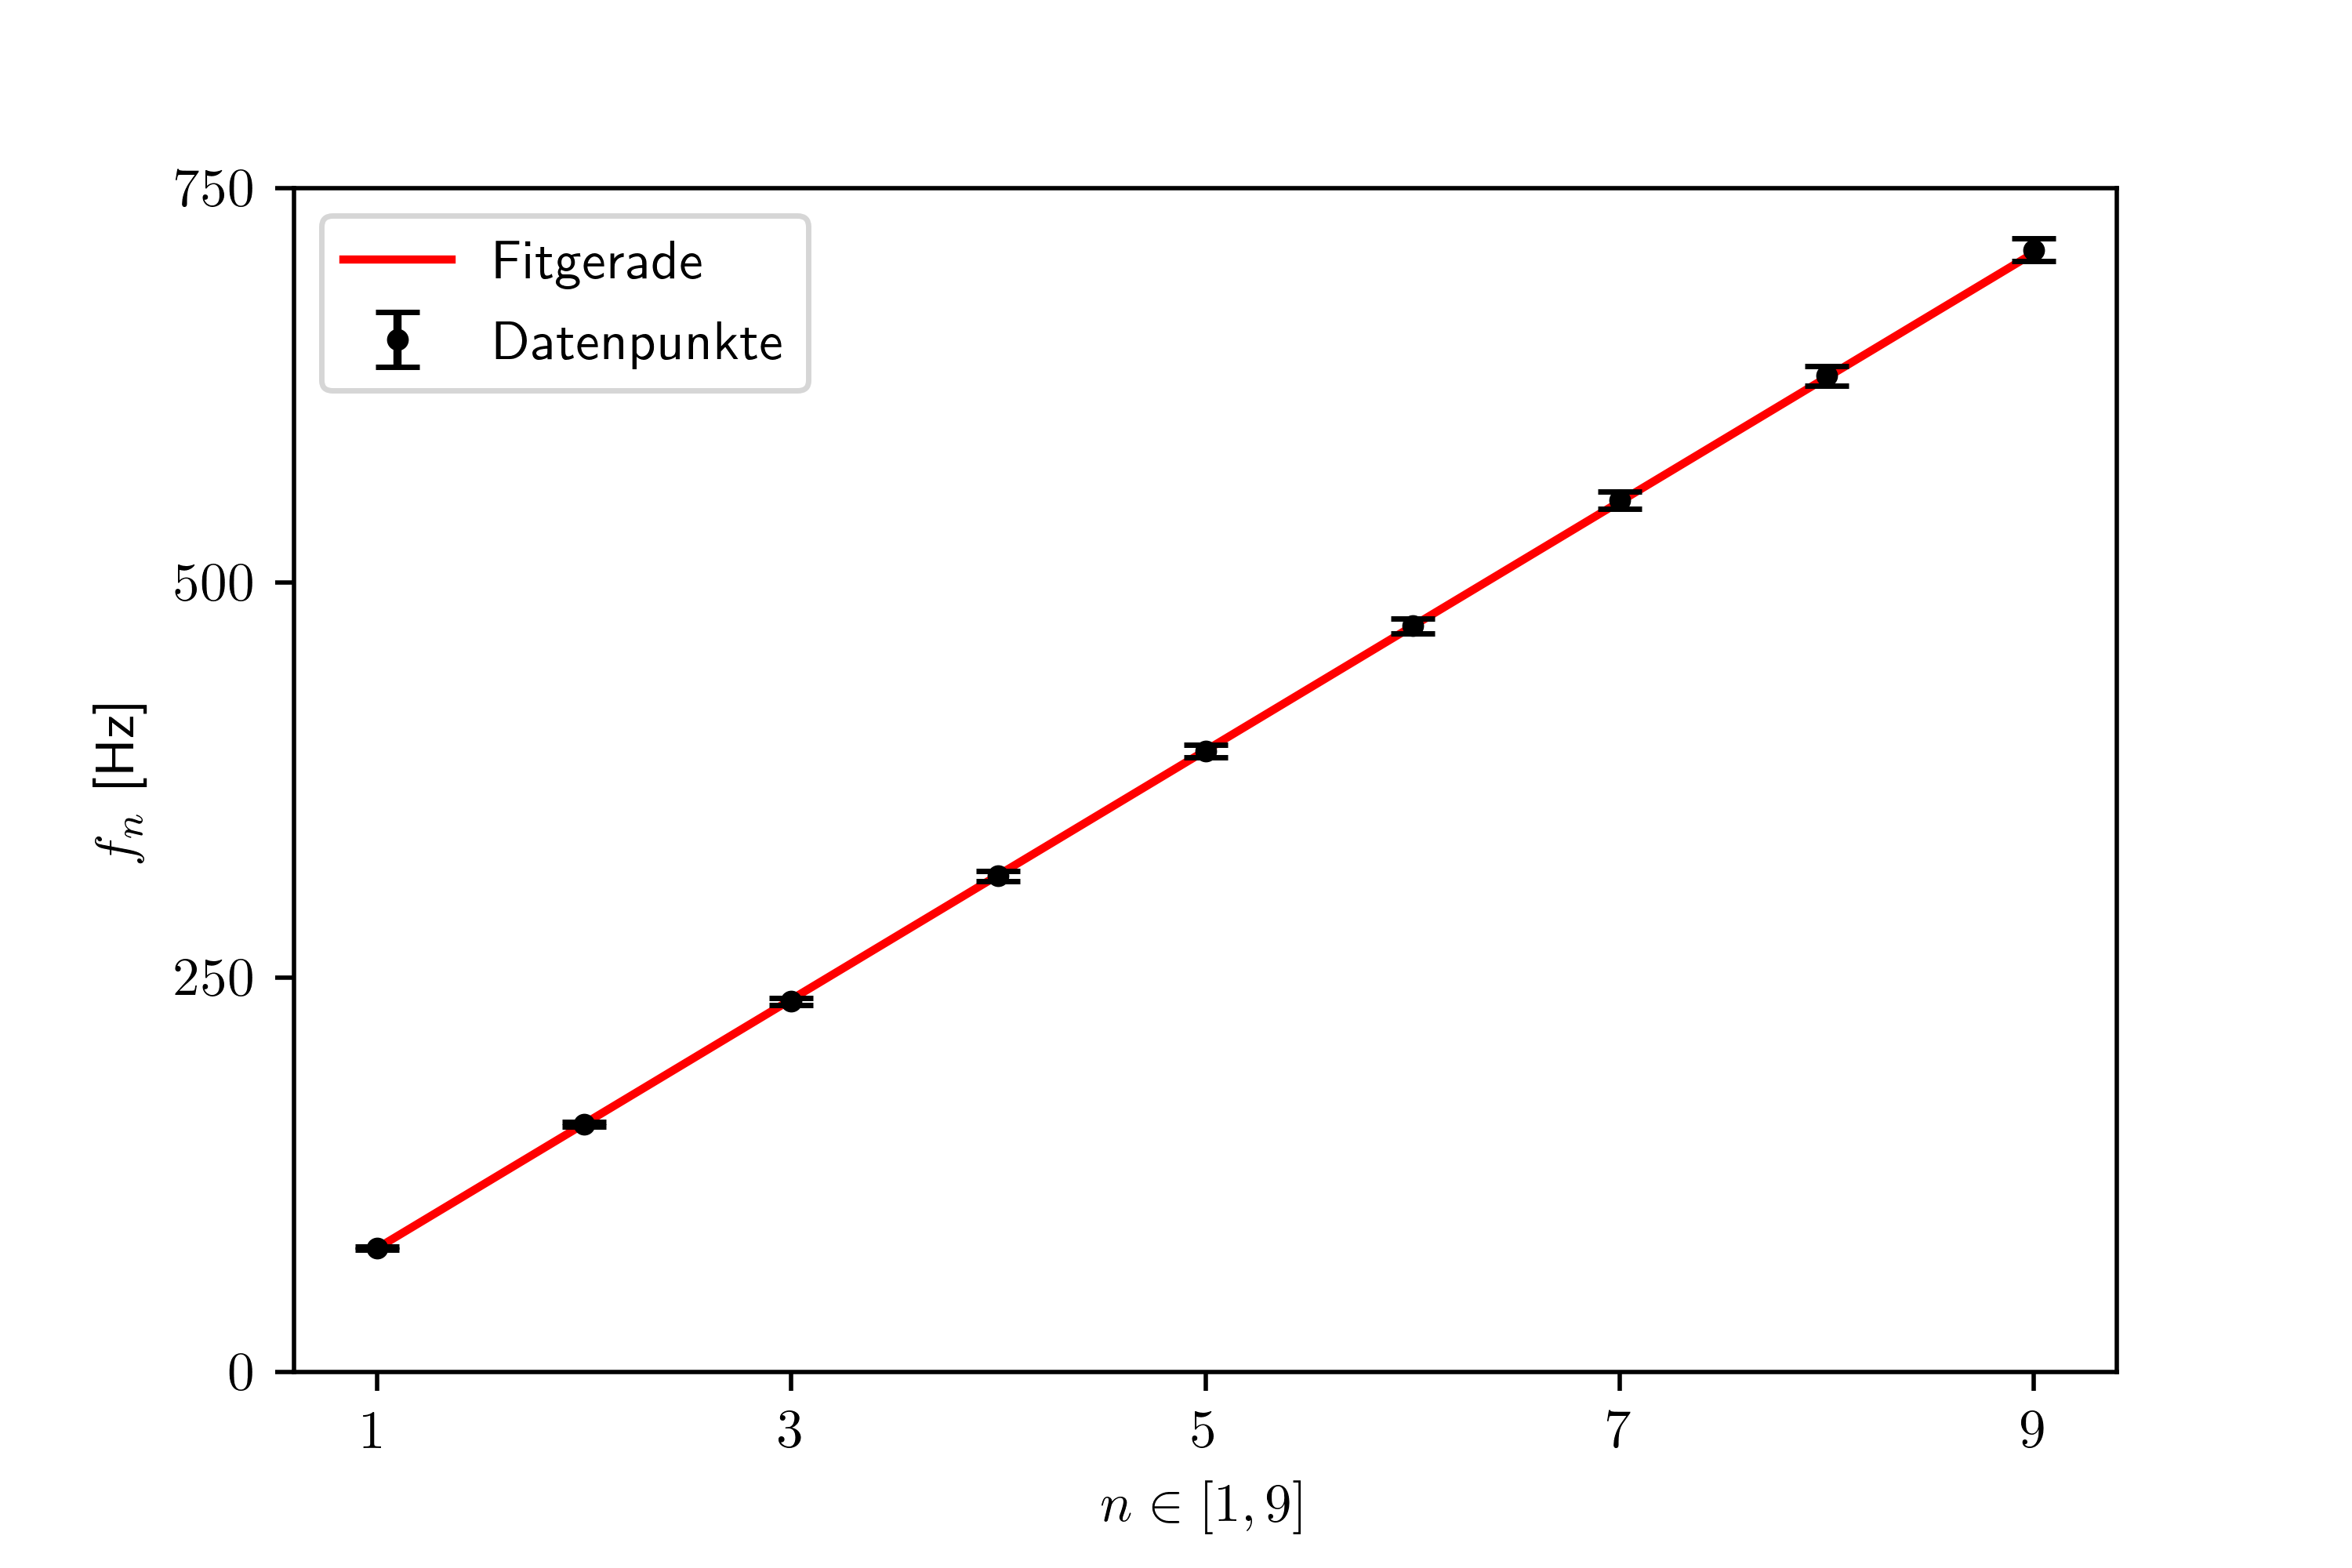
\includegraphics[width=350pt]{fotos/gpr1/Regression_A1.png}			% einfügen des Bildes/ mit width Bildbreite einstellen
		\caption{lineare Regression zwischen Resonanzfrequenz und unterschiedlichen Bäuchen.}							% Bildunterschrift
		\label{Abb: Regression 1}							% für Textverweise
	\end{figure}
\begin{figure}[!ht]
	\centering									% Bild Zentrierung
	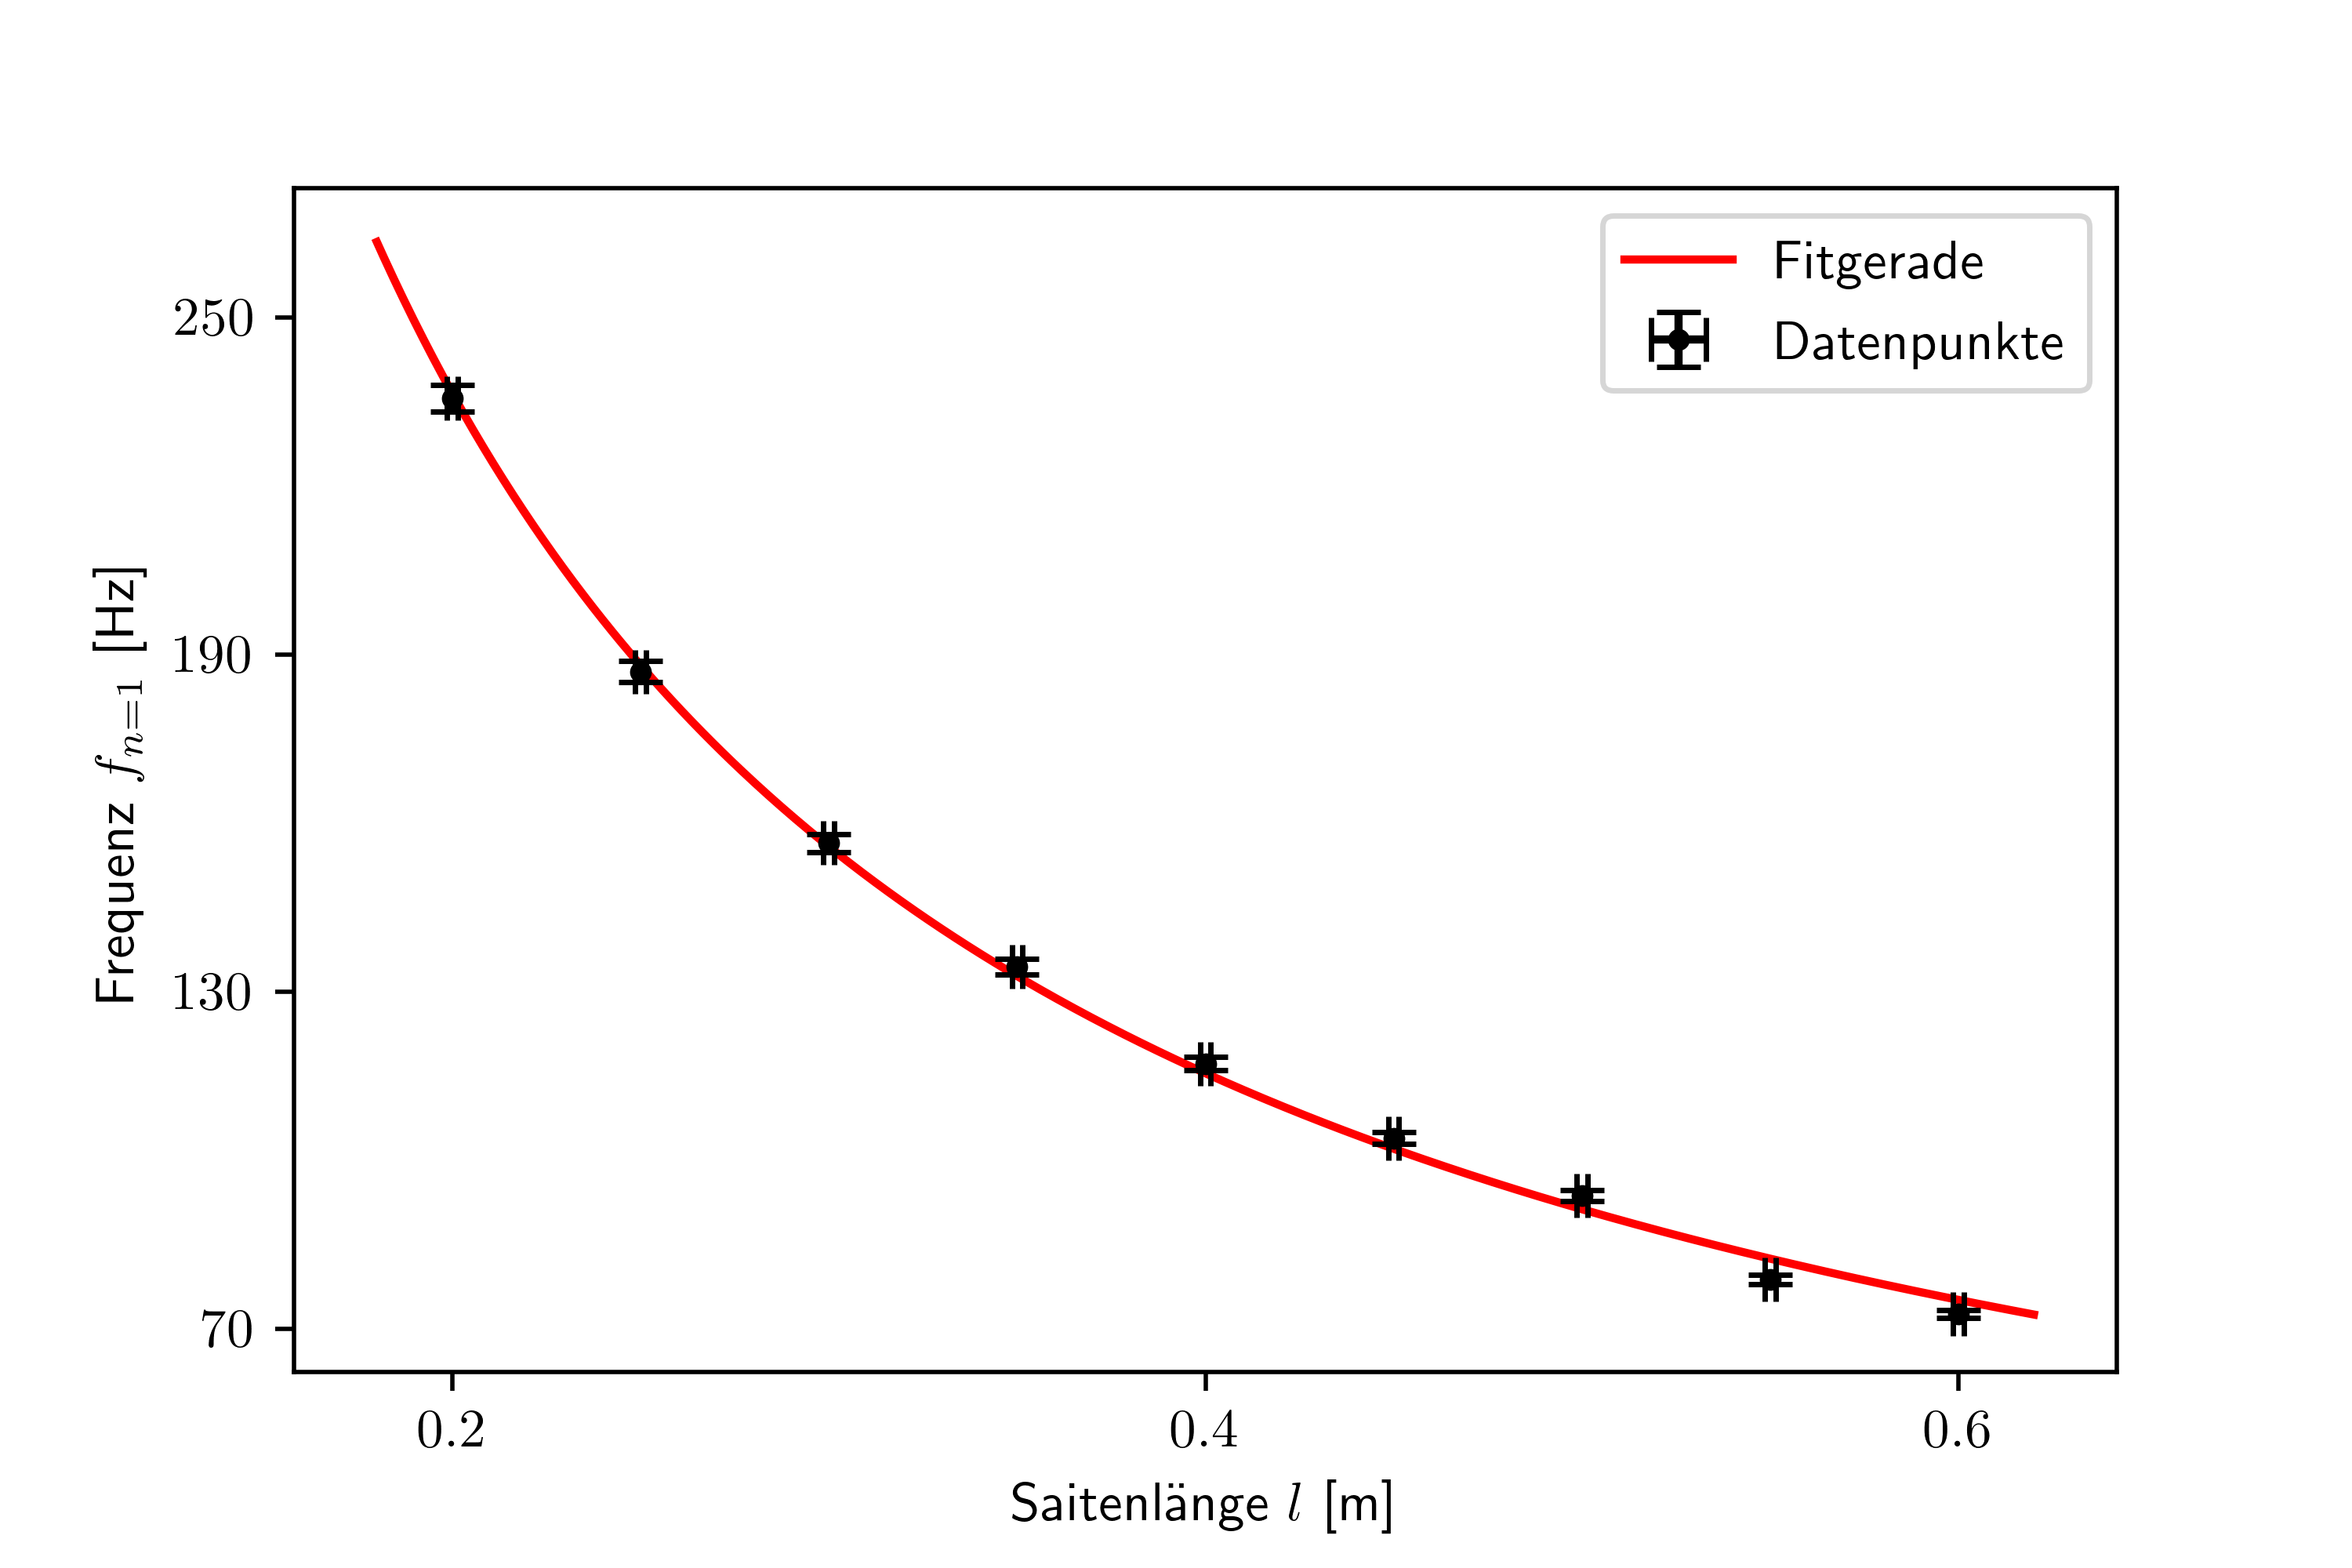
\includegraphics[width=350pt]{fotos/gpr1/Regression_A2.png}			% einfügen des Bildes/ mit width Bildbreite einstellen
	\caption{lineare Regression zwischen Resonanzfrequenz $f_{n=1}$ und der Saitenlänge $l$ }							% Bildunterschrift
	\label{Abb: Regression 2}							% für Textverweise
\end{figure}
\newpage
\begin{figure}[!ht]
	\centering									% Bild Zentrierung
	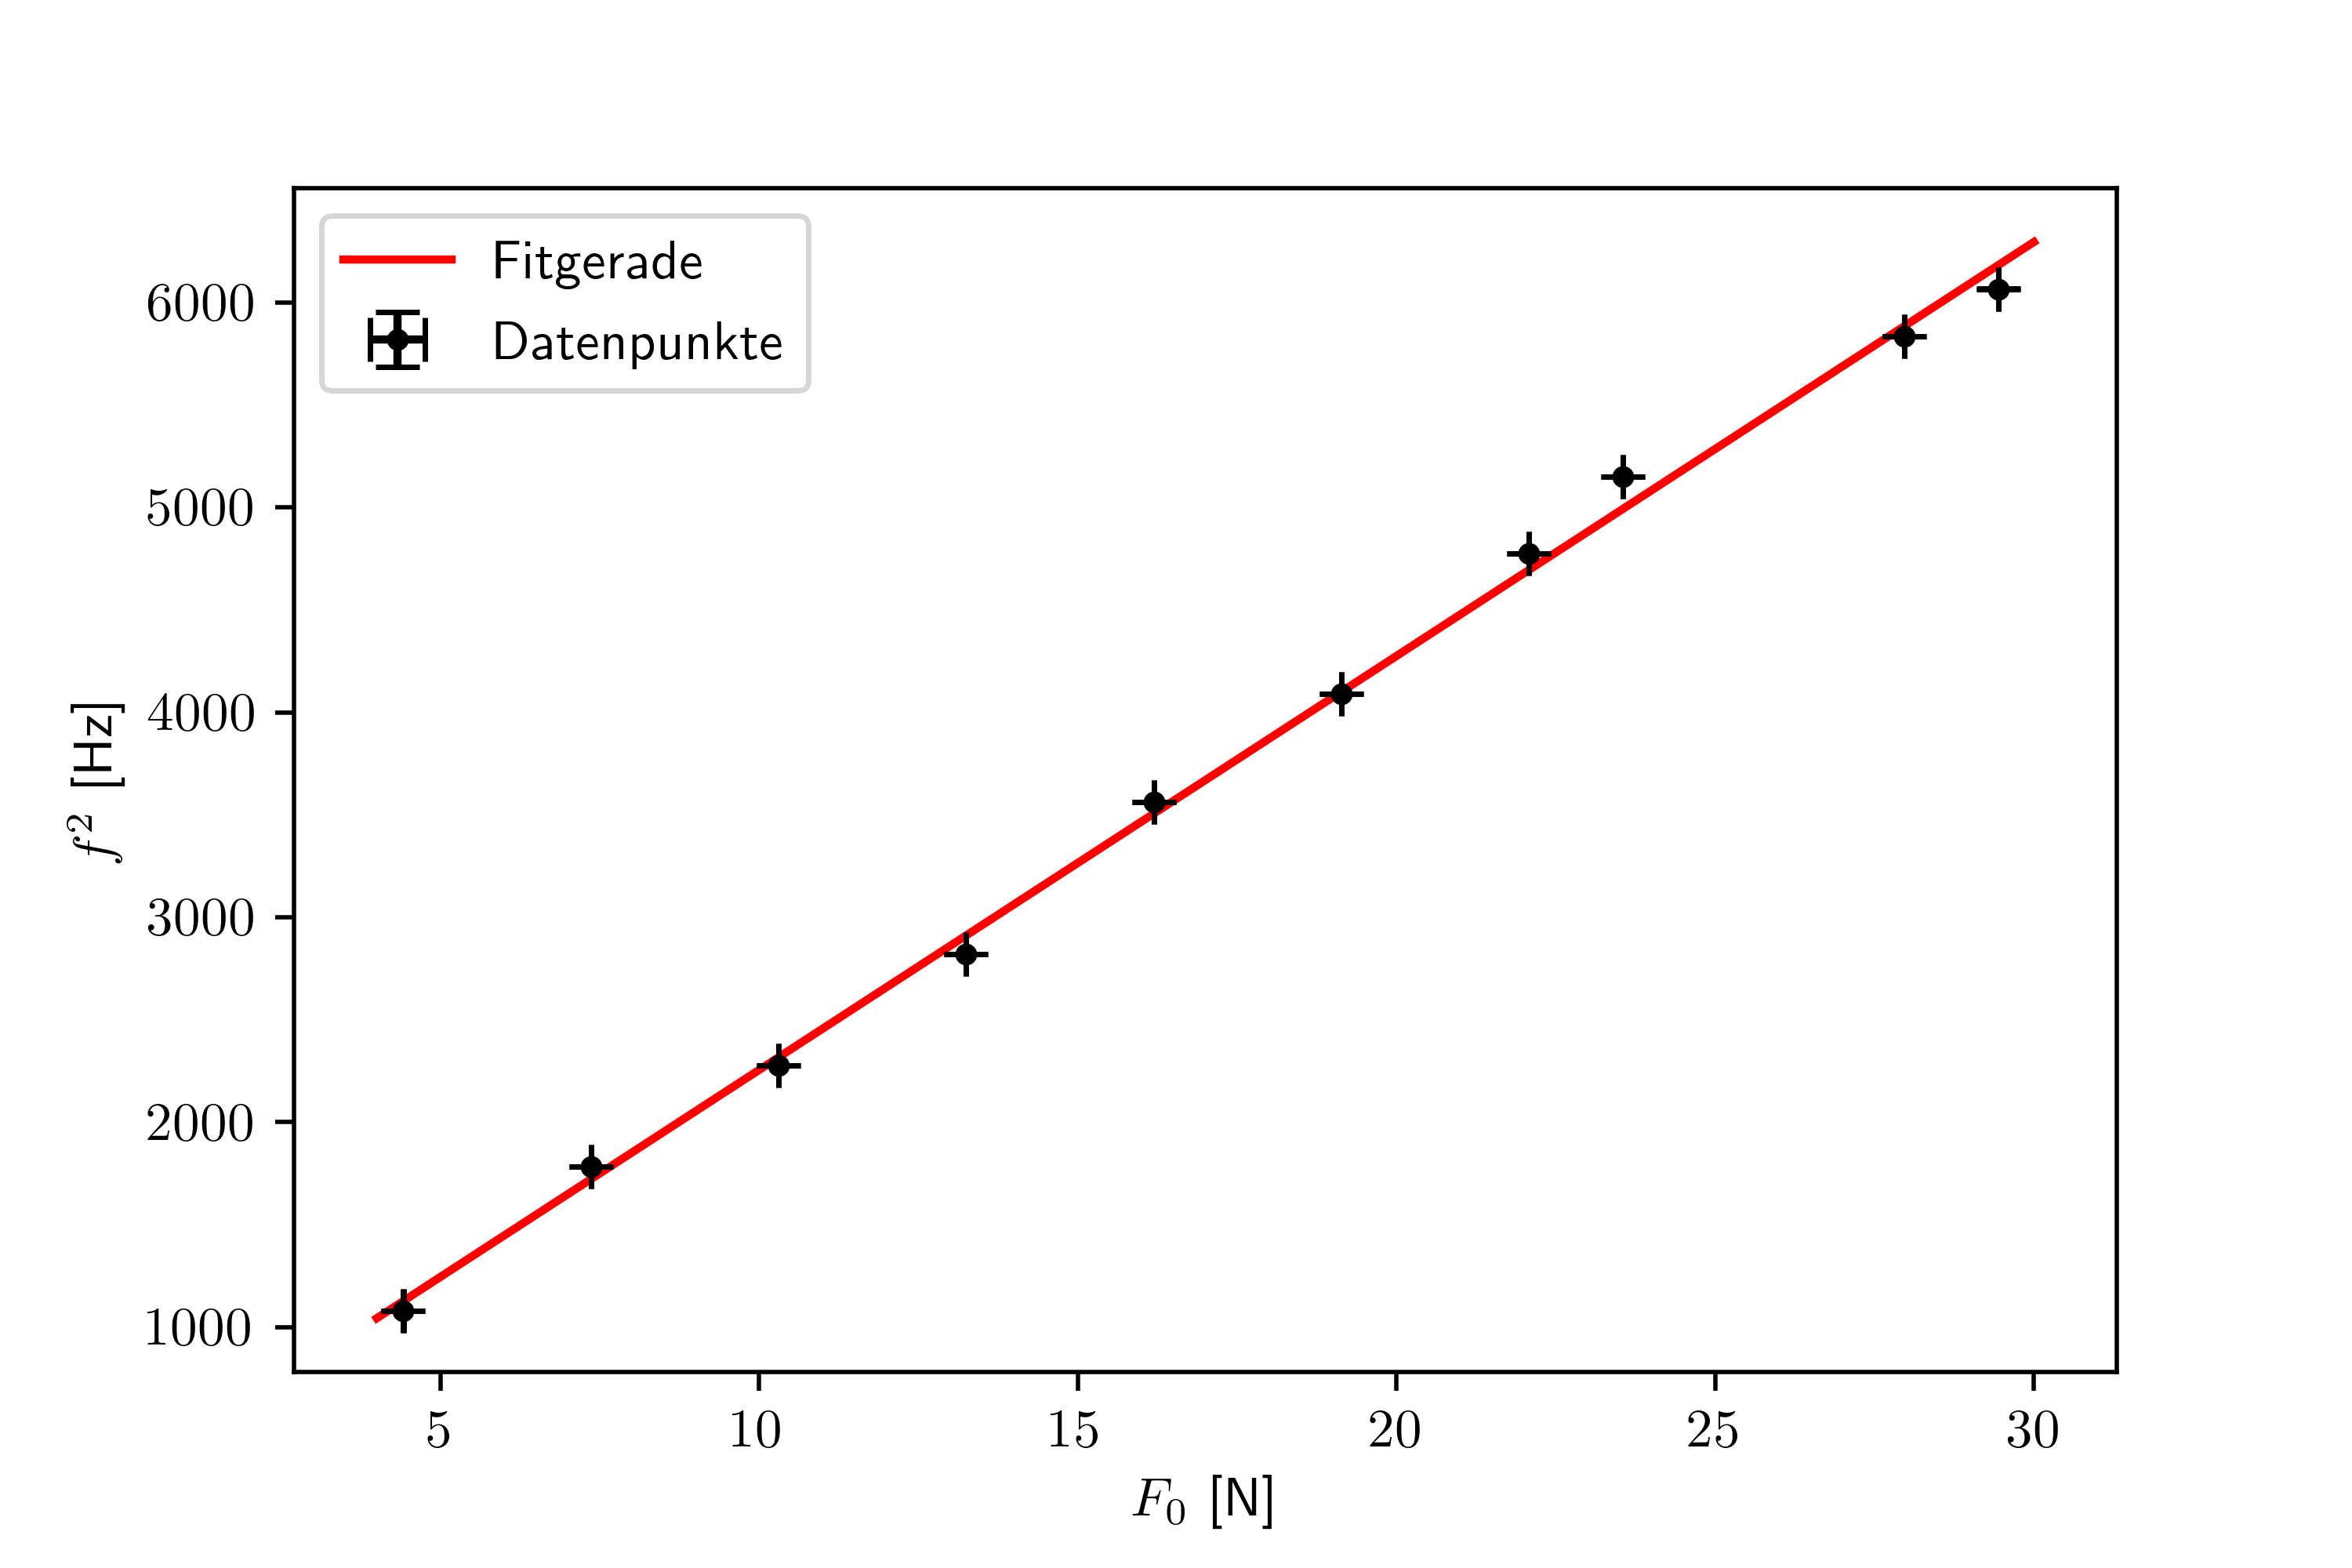
\includegraphics[width=350pt]{fotos/gpr1/Regression_A3.png}			% einfügen des Bildes/ mit width Bildbreite einstellen
	\caption{lineare Regression zwischen Resonanzfrequenz $ f $ und unterschliedlichen Zugspannungen $ F_{0} $.}							% Bildunterschrift
	\label{Abb: Regression 3}							% für Textverweise
\end{figure}
\subsection{Angaben am Versuchsplatz}

\begin{figure}[!ht]
	\centering									% Bild Zentrierung
	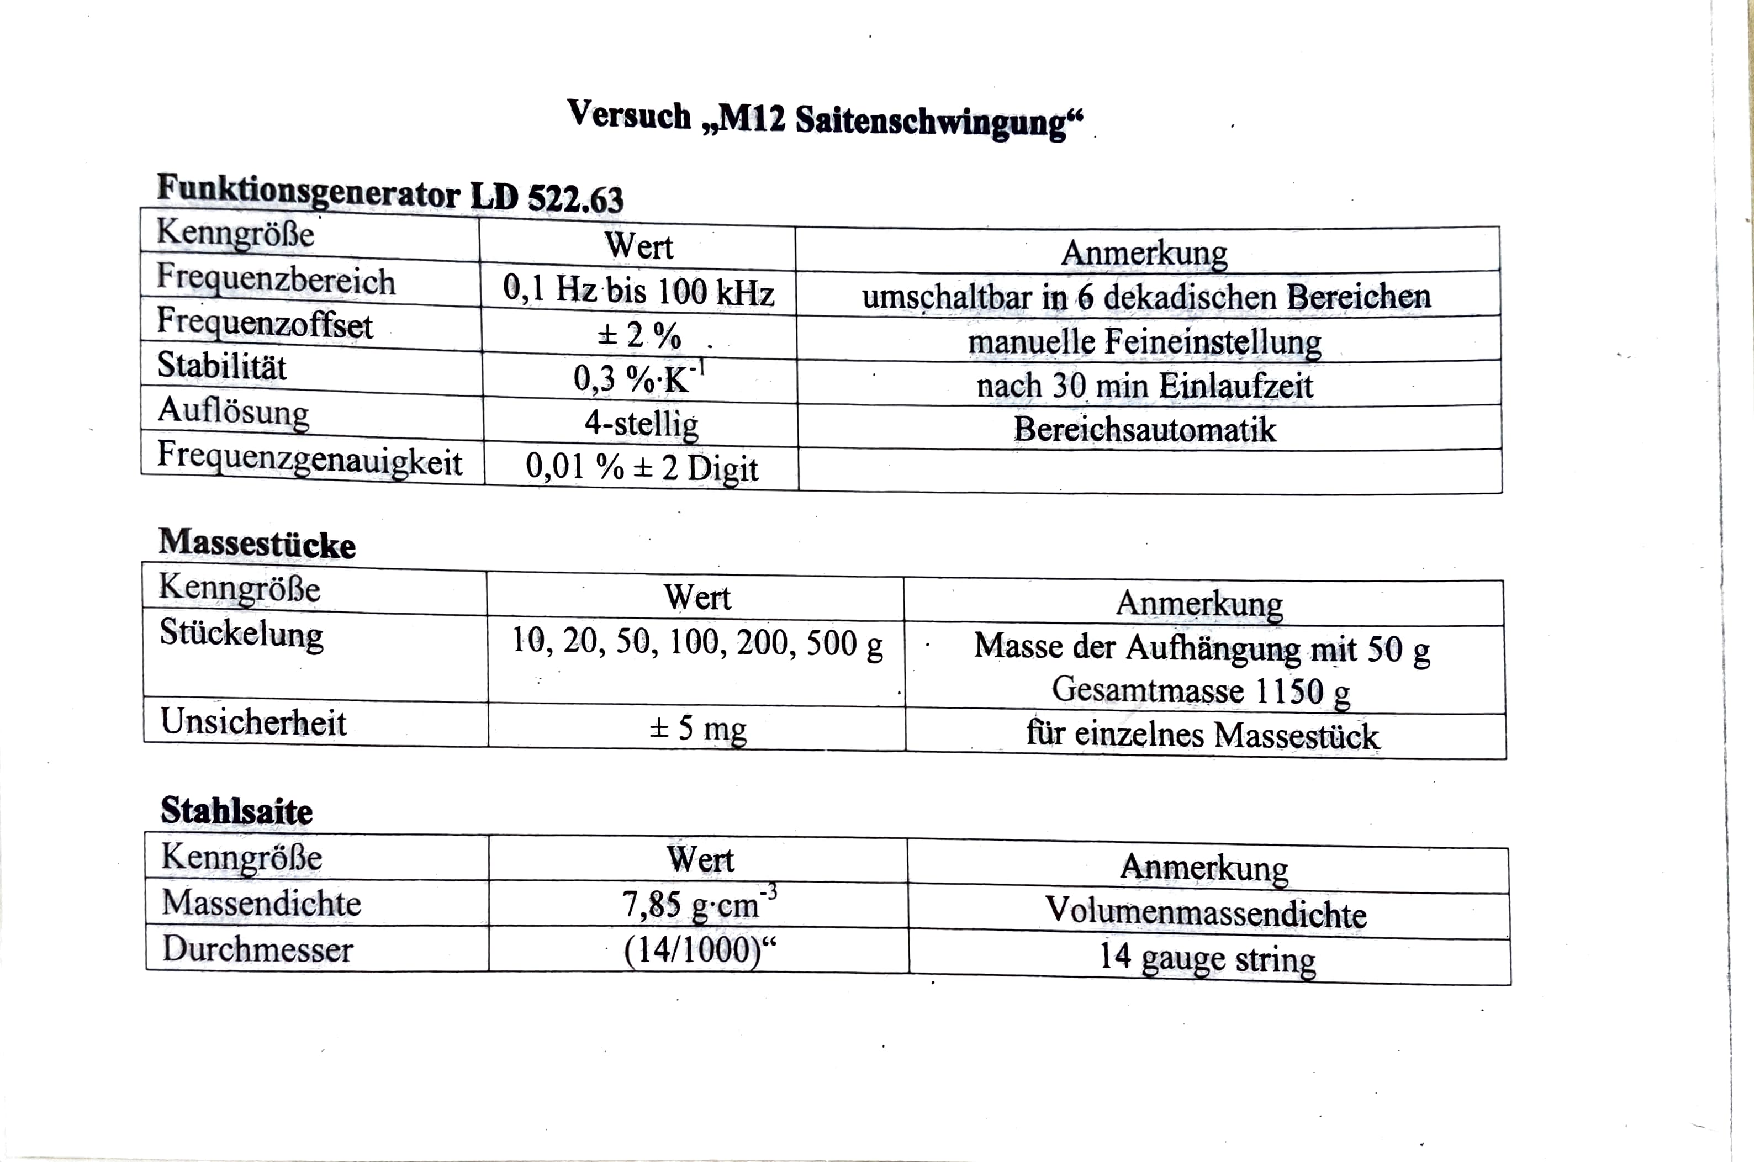
\includegraphics[width=300pt]{fotos/gpr1/Versuch.M12.pdf}			% einfügen des Bildes/ mit width Bildbreite einstellen
	\caption{Angaben am Versuchsplatz für den Funktionsgenerator, die Massestücke und die Stahlsaite}							% Bildunterschrift
	\label{Abb: Agaben}							% für Textverweise
\end{figure}

\newpage


	\newpage
	
	\printbibliography[title={Quellenverzeichnis}]
	
	
\end{document}